\newtheorem{myDefinition}{Definition}
\newtheorem{myTheorem}{Theorem}
\newtheorem{myLemma}{Lemma}

% other definitions
% basic matrices
\newcommand{ \A }[1]        { \textbf{A}^{\mathrm{\!#1}} }  % pull in exponent

% inverses
\newcommand{ \Ap }[0]       { \A{\sym} }
\newcommand{ \Ainv }[0]     { \A{-1} }
\newcommand{ \Ainvs }[0]    { \A{-*} }
\newcommand{ \AinvL }[0]    { \A{-L} }
\newcommand{ \AinvR }[0]    { \A{-R} }

% projectors
\newcommand{ \ApA }[0]      { \A{\sym}\A{} }
\newcommand{ \AAp }[0]      { \A{}\,\A{\sym} }

% matrix vector products
\newcommand{ \Ax }[0]       { \A{}\,x }
\newcommand{ \Axez }[0]     { \Ax = \zero }
\newcommand{ \Axey }[0]     { \Ax = y }
\newcommand{ \Axeb }[0]     { \Ax = b }
\newcommand{ \Asyex }[0]    { \A{*}y = x }
\newcommand{ \Axmb }[0]     { \Ax - b }
\newcommand{ \Axls }[0]     { \A{}\,x_{LS} }
\newcommand{ \Avk }[0]      { \A{}\,{\bl{ v_{k} }} }

% membership
\newcommand{ \aicmm }[0]    { \A{} \in \cmplxmm }
\newcommand{ \aicmn }[0]    { \A{} \in \cmplxmn }
\newcommand{ \aicmnr }[0]   { \A{} \in \cmplxmnr }
\newcommand{ \aicmmm }[0]   { \A{} \in \cmplxmmm }
\newcommand{ \aicmnm }[0]   { \A{} \in \cmplxmnm }
\newcommand{ \aicmnn }[0]   { \A{} \in \cmplxmnn }

\newcommand{ \airmn }[0]    { \A{} \in \realxmn }
\newcommand{ \airmnr }[0]   { \A{} \in \realxmnr }
\newcommand{ \airmmm }[0]   { \A{} \in \realmmm }

\newcommand{ \xicn }[0]     { x    \in \cmplxn }

% product matrices
\newcommand{ \wx }[1]       { \A{#1}  \A{} }
\newcommand{ \wy }[1]       { \A{} \, \A{#1} }

% product matrix equations
\newcommand{ \wxe }[1]      { \W{V} = \wx{#1} }
\newcommand{ \wye }[1]      { \W{U} = \wy{#1} }

\newcommand{ \wv }[0]       { \W{V} }
\newcommand{ \wu }[0]       { \W{U} }

% SVD equations
\newcommand{ \aesvd }[1]    { \A{}  = \svd{ #1 } }
\newcommand{ \aaesvd }[1]   { \A{} &= \svd{ #1 } }
\newcommand{ \aetsvd }[1]   { \A{}  = \bur{}\, \ess{}\, \bvr{ #1 } }

% SVD transpose equations
\newcommand{ \aesvdt }[1]   { \A{ #1 }  = \svdt{ #1 } }
\newcommand{ \aaesvdt }[1]  { \A{ #1 } &= \svdt{ #1 } }

% Moore-Penrose pseudoinverse equations
\newcommand{ \apempp }[1]   { \Ap   = \mpp{ #1 } }
\newcommand{ \apaempp }[1]  { \Ap  &= \mpp{ #1 } }

\newcommand{ \apemppfr }[1] { \Ap   = \mppfr{ #1 } }
\newcommand{ \apaemppfr }[1]{ \Ap  &= \mppfr{ #1 } }

% combos
\newcommand{ \ax }[0]       { \A{}\,\X{} }  % pull in 

\endinput
\def\tr{\text{tr}}
\def\spn {span}
\def\sgn {\text{sgn }}
%\def\span{span}
\def\mx{max}
\def\dm{dim}
\def\adj{adj}
\def\Arg{Arg}
\def\rref{rref}
\def\ns{null space}

\endinput
\input{\pathname/"bold letters"}
%% shades of gray
\definecolor{darkgray}{gray}{0.25}
\definecolor{medgray} {gray}{0.75}
\definecolor{ltgray}  {gray}{0.90}
\definecolor{vltgray} {gray}{0.95}

%\definecolor{rangecolor} {blue}
%\definecolor{nullcolor}  {red}

%% basic color directives
\newcommand{ \bl }[1]        {{\color{blue}   {#1}}}
\newcommand{ \bk }[1]        {{\color{black}  {#1}}}
\newcommand{ \rd }[1]        {{\color{red}    {#1}}}
\newcommand{ \gr }[1]        {{\color{green}  {#1}}}
\newcommand{ \pr }[1]        {{\color{purple} {#1}}}
\newcommand{ \mg }[1]        {{\color{medgray}{#1}}}

%% numbers blue
\newcommand{ \bzero }[0]     { \bl{ 0 } }
\newcommand{ \bone }[0]      { \bl{ 1 } }
\newcommand{ \btwo }[0]      { \bl{ 2 } }
\newcommand{ \bthree }[0]    { \bl{ 3 } }
\newcommand{ \bfour }[0]     { \bl{ 4 } }
\newcommand{ \bfive }[0]     { \bl{ 5 } }
\newcommand{ \bsix }[0]      { \bl{ 6 } }
\newcommand{ \bseven }[0]    { \bl{ 7 } }
\newcommand{ \beight }[0]    { \bl{ 8 } }
\newcommand{ \bnine }[0]     { \bl{ 9 } }
\newcommand{ \bminus }[0]    { \bl{ - } }
\newcommand{ \bstar }[0]     { \bl{ * } }
\newcommand{ \bi }[0]        { \bl{ i } }
\newcommand{ \bmone }[0]     { \bl{-1 } }
\newcommand{ \bmi }[0]       { \bl{-i } }
\newcommand{ \bmo }[0]       { \bl{-1 } }

\newcommand{ \bdots }[0]     { \bl{ \dots } }


%% numbers red
\newcommand{ \rzero }[0]     { \rd{ 0 } }
\newcommand{ \rone }[0]      { \rd{ 1 } }
\newcommand{ \rtwo }[0]      { \rd{ 2 } }
\newcommand{ \rthree }[0]    { \rd{ 3 } }
\newcommand{ \rfour }[0]     { \rd{ 4 } }
\newcommand{ \rfive }[0]     { \rd{ 5 } }
\newcommand{ \rsix }[0]      { \rd{ 6 } }
\newcommand{ \rseven }[0]    { \rd{ 7 } }
\newcommand{ \reight }[0]    { \rd{ 8 } }
\newcommand{ \rnine }[0]     { \rd{ 9 } }
\newcommand{ \rminus }[0]    { \rd{ - } }
\newcommand{ \rstar }[0]     { \rd{ * } }
\newcommand{ \rmone }[0]     { \rd{-1 } }

\newcommand{ \rdots }[0]     { \rd{ \dots } }

%% numbers medium gray
\newcommand{ \gzero }[0]     { \mg{ 0 } }
\newcommand{ \gone }[0]      { \mg{ 1 } }
\newcommand{ \gtwo }[0]      { \mg{ 2 } }
\newcommand{ \gthree }[0]    { \mg{ 3 } }
\newcommand{ \gfour }[0]     { \mg{ 4 } }
\newcommand{ \gfive }[0]     { \mg{ 5 } }
\newcommand{ \gsix }[0]      { \mg{ 6 } }
\newcommand{ \gseven }[0]    { \mg{ 7 } }
\newcommand{ \geight }[0]    { \mg{ 8 } }
\newcommand{ \gnine }[0]     { \mg{ 9 } }
\newcommand{ \gminus }[0]    { \mg{ - } }
\newcommand{ \goplus }[0]    { \mg{ \oplus } }

%% numbers black
\newcommand{ \bs }[0]        { {\bk{*}} }
\newcommand{ \bkzero }[0]    { {\bk{0}} }

% nums
\newcommand{ \bnum }[0]      { \bl{ \num } }
\newcommand{ \rnum }[0]      { \rd{ \num } }
\newcommand{ \gnum }[0]      { \mg{ \num } }

\endinput  %  -  -  -  -  -  -  -  -  -  -  -  -  -  -  -  -  -  -  -  -
\input{\fullpath/"convolution kernels"}
\providecommand{\paren}[1] { \left(  #1 \right) }
\providecommand{\inner}[1] { \langle #1 \rangle }
\providecommand{\brac}[1]  { \left[  #1 \right] }
\providecommand{\lst}[1]   { \left\{ #1 \right\} }

\endinput
\input{\fullpath/"dirac definitions"}
\input{\pathname/"example a matrices"}
\input{\pathname/"example b matrices"}
\input{\pathname/"example c matrices"}
% range and null space
\newcommand{ \atomrng }[0]   { \mathcal{R} }
\newcommand{ \atomnll }[0]   { \mathcal{N} }

\newcommand{ \rng }[1]       { \atomrng \! \paren{ #1 } }
\newcommand{ \nll }[1]       { \atomnll \! \paren{ #1 } }

\newcommand{ \rnga }[1]      { \rng{ \A{ #1 } } }
\newcommand{ \nlla }[1]      { \nll{ \A{ #1 } } }

\newcommand{ \brnga }[1]     { \bl{ \rnga{ #1 } } }
\newcommand{ \rnlla }[1]     { \rd{ \nlla{ #1 } } }
\newcommand{ \gnlla }[1]     { \mg{ \nlla{ #1 } } }

% orthogonal decomposition
\newcommand{ \decompdo }[1]  { \rnga{ #1 }  \oplus \nlla{} }
\newcommand{ \decompco }[1]  { \rnga{}      \oplus \nlla{ #1 } }

\newcommand{ \cdecompdo }[1] { \brnga{ #1 } \oplus \rnlla{} }
\newcommand{ \cdecompco }[1] { \brnga{}     \oplus \rnlla{ #1 } }

% FTOLA
\newcommand{ \ftolado }[1]   { \cmplxn =  \decompdo{ #1 } }
\newcommand{ \ftolaco }[1]   { \cmplxm =  \decompco{ #1 } }

\newcommand{ \cftolado }[1]  { \cmplxn = \cdecompdo{ #1 } }
\newcommand{ \cftolaco }[1]  { \cmplxm = \cdecompco{ #1 } }

% rank plus nullity
\newcommand{ \rpn }[0]       {\text{rank}\paren{\A{}} + \text{dim}\paren{\text{nullity}\paren{\A{}}}}

% projectors
\newcommand{ \pra }[0]       { \textbf{P}_{\brnga{}} }
\newcommand{ \pras }[0]      { \textbf{P}_{\brnga{*}} }
\newcommand{ \pnas }[0]      { \textbf{P}_{\rnlla{*}} }
\newcommand{ \pna }[0]       { \textbf{P}_{\rnlla{}} }

\endinput  %  -  -  -  -  -  -  -  -  -  -  -  -  -  -  -  -  -  -  -  -
\input{\fullpath/"gellmann definitions"}
\input{\fullpath/"jordan forms"}
% Hilbert matrices
\newcommand{ \hilberttwo }[0]   { \mat{cc}{ 1&\half\\\half&\recip{3}} }

\newcommand{ \hilbertthree }[0] { \mat{ccc}
{ 
1         & \half     & \recip{3} \\ 
\half     & \recip{3} & \recip{4} \\ 
\recip{3} & \recip{4} & \recip{5} 
}}

\newcommand{ \numa }[0] { \sqrt{ \half + \recip{\sqrt{13}} } }
\newcommand{ \numb }[0] { \sqrt{ \half - \recip{\sqrt{13}} } }

\newcommand{ \hilberttwoU }[0] {
\mat{rr}{ {\bl{ \numa }} & {\bl{ -\numb }} \\ {\bl{ \numb }} & {\bl{ \numa }} } }

\newcommand{ \hilberttwoVT }[0] {
\mat{rr}{ {\bl{ \numa }} & {\bl{ \numb }} \\ {\bl{ -\numb }} & {\bl{ \numa }} } }

\newcommand{ \hilberttwoS }[0] {
\recip{6}
\mat{rr}{ 4 + \sqrt{13} & 0 \\ 0 & 4 - \sqrt{13} } }

\newcommand{\abs}[1]         {\left|#1\right|}
\providecommand{\norm}[1]    {\left\lVert#1\right\rVert}
\providecommand{\normo}[1]   {\left\lVert#1\right\rVert_{1}}
\providecommand{\normt}[1]   {\left\lVert#1\right\rVert_{2}}
\providecommand{\norminf}[1] {\left\lVert#1\right\rVert_\infty}
\providecommand{\normp}[1]   {\left\lVert#1\right\rVert_{p}}
\providecommand{\normf}[1]   {\left\lVert#1\right\rVert_F}

\providecommand{\norms}[1]   {\left\lVert#1\right\rVert^{2}}
\providecommand{\normos}[1]  {\left\lVert#1\right\rVert_{1}^{2}}
\providecommand{\normts}[1]  {\left\lVert#1\right\rVert_{2}^{2}}
\providecommand{\norminfs}[1]{\left\lVert#1\right\rVert_\infty^{2}}
\providecommand{\normps}[1]  {\left\lVert#1\right\rVert_{p}^{2}}
\providecommand{\normfs}[1]  {\left\lVert#1\right\rVert_F^{2}}

\endinput
\newcommand{\boxone} {$\boxed{1}$}

\endinput
% reciprocals
\newcommand{\recip}[1]    {\frac{1}{#1}}
\newcommand{\recipp}[1]   {\paren{ \frac{1}{#1} }}
\newcommand{\recips}[1]   {\frac{1}{\sqrt{#1}}}
\newcommand{\half}[0]     {\recip{2}}
\newcommand{\third}[0]    {\recip{3}}
\newcommand{\quarter}[0]  {\recip{4}}

\newcommand{\rstwo}[0]    {\recip{\sqrt{2}}}
\newcommand{\rsthree}[0]  {\recip{\sqrt{3}}}
\newcommand{\rsfive}[0]   {\recip{\sqrt{5}}}
\newcommand{\rssix}[0]    {\recip{\sqrt{6}}}
\newcommand{\rsthirty}[0] {\recip{\sqrt{30}}}

\newcommand{\rsmtwo}[0]   {\frac{-1}{\sqrt{2}}}
\newcommand{\rsmthree}[0] {\frac{-1}{\sqrt{3}}}
\newcommand{\rsmsix}[0]   {\frac{-1}{\sqrt{6}}}

% 2, ... over
\newcommand{\rstfive}[0]   {\frac{2} {\sqrt{5}}}
\newcommand{\rstsix}[0]    {\frac{2} {\sqrt{6}}}
\newcommand{\rstthirty}[0] {\frac{2} {\sqrt{30}}}
\newcommand{\rsfthirty}[0] {\frac{5} {\sqrt{30}}}
\newcommand{\rsmtfive}[0]  {\frac{-2} {\sqrt{5}}}
\newcommand{\rsmtthirty}[0]{\frac{-2} {\sqrt{30}}}

% colored versions
\newcommand{\brstwo}[0]    {{\bl{ \rstwo }}}
\newcommand{\brsmtwo}[0]   {{\bl{ \rsmtwo }}}
\newcommand{\brsthree}[0]  {{\bl{ \rsthree }}}
\newcommand{\brsmthree}[0] {{\bl{ \rsmthree }}}

\newcommand{\brsthirty}[0] {{\bl{ \rsthirty }}}
\newcommand{\brsmtthirty}[0]{{\bl{\rsmtthirty }}}
\newcommand{\brstthirty}[0]{{\bl{ \rstthirty }}}
\newcommand{\brsfthirty}[0]{{\bl{ \rsfthirty }}}

\newcommand{\brssix}[0]    {{\bl{ \rssix }}}
\newcommand{\brsmsix}[0]   {{\bl{ \rsmsix }}}
\newcommand{\brstsix}[0]   {{\bl{ \rstsix }}}

\newcommand{\rrstwo}[0]    {{\rd{ \rstwo }}}
\newcommand{\rrsmtfive}[0] {{\rd{ \rsmtfive }}}
\newcommand{\rrsfive}[0]   {{\rd{ \rsfive }}}
\newcommand{\rrssix}[0]    {{\rd{ \rssix }}}
\newcommand{\rrsmsix}[0]   {{\rd{ \rsmsix }}}
\newcommand{\rrstsix}[0]   {{\rd{ \rstsix }}}


\endinput
% bys
\newcommand{\by}[2]      {#1 \times #2}
\newcommand{\byy}[1]     {#1 \times #1}
\newcommand{\bymn}[0]    {\by{m}{n}}
\newcommand{\bymm}[0]    {\byy{m}}
\newcommand{\bynn}[0]    {\byy{n}}
\newcommand{\bynm}[0]    {\by{n}{m}}
\newcommand{\bymr}[0]    {\by{m}{\rho}}
\newcommand{\byrn}[0]    {\by{\rho}{n}}

% vector spaces
\newcommand{\real}[1]    {\mathbb{R}^{#1}}
\newcommand{\cmplx}[1]   {\mathbb{C}^{#1}}
\newcommand{\either}[1]  {\cmplx{#1}}
\newcommand{\ir}[0]      {\in\real{}}
\newcommand{\ic}[0]      {\in\cmplx{}}
\newcommand{\icm}[0]     {\in\cmplxm}
\newcommand{\icn}[0]     {\in\cmplxn}
\newcommand{\icmn}[0]    {\in\cmplxmn}
\newcommand{\irmn}[0]    {\in\realmn}
\newcommand{\icmnr}[0]   {\in\cmplxmnr}
\newcommand{\ints}[0]    {\mathbb{Z}}
\newcommand{\natnum}[0]  {\mathbb{N}}

\newcommand{\iints}[0]   {\in \mathbb{Z}}
\newcommand{\inatnum}[0] {\in \mathbb{N}}

\newcommand{\realall}[3] {\real{\by{#1}{#2}}_{#3} }
\newcommand{\cmplxall}[3]{\cmplx{\by{#1}{#2}}_{#3} }

\newcommand{\realn}[0]   {\real{n}}
\newcommand{\realm}[0]   {\real{m}}
\newcommand{\realmn}[0]  {\real{\bymn}}
\newcommand{\realnn}[0]  {\real{\byy{n}}}
\newcommand{\realmm}[0]  {\real{\byy{m}}}
\newcommand{\realmmr}[0] {\real{\byy{m}}_{\rho}}
\newcommand{\realmmm}[0] {\realmm_{m}}

\newcommand{\cmplxn}[0]  {\cmplx{n}}
\newcommand{\cmplxm}[0]  {\cmplx{m}}
\newcommand{\cmplxnn}[0] {\cmplx{\byy{n}}}
\newcommand{\cmplxmm}[0] {\cmplx{\byy{m}}}
\newcommand{\cmplxmn}[0] {\cmplx{\bymn}}
\newcommand{\cmplxmr}[0] {\cmplx{\bymr}}
\newcommand{\cmplxrn}[0] {\cmplx{\byrn}}
\newcommand{\cmplxmnr}[0]{\cmplx{\bymn}_{\rho}}
\newcommand{\cmplxmmm}[0]{\cmplxmm_{m}}
\newcommand{\cmplxmnm}[0]{\cmplxmn_{m}}
\newcommand{\cmplxnnr}[0]{\cmplxnn_{\rho}}
\newcommand{\cmplxmnn}[0]{\cmplxmn_{n}}

% spans
\newcommand{\spn}[1]     {\text{sp\,} \lst{ #1 }}


\endinput  %  -  -  -  -  -  -  -  -  -  -  -  -  -  -  -  -  -  -  -  -
\input{\pathname/"least squares"}
\input{\pathname/"matrix basics"}
\input{\pathname/"matrix decompositions"}
\input{\pathname/"sigma matrices"}
\input{\pathname/"svd forms"}
\section{Vectors}
\label{sec:vectors}
Row vectors are fun targets for the \svdl. It's very easy to visualize the domain and codomain.

%%
\subsection{\vv s}
Consider the \vv \ below:
\begin{equation}
  v=\mat{c}{1\\\frac{1}{2}}.
  \label{eq:cases:2v}
\end{equation}
Hopefully the rank of the system is obvious:
\begin{equation}
  \rho = \min\lst{m,n}= \min\lst{2,1} = 1
\end{equation}

The decomposition will have these form factors
\begin{equation}
  \begin{array}{ccccc}
  \A{} &=& \Y{} & \sig{} & \X{T}\\
  \by{m}{n}&=&\paren{\by{m}{m}}&\paren{\by{m}{n}}&\paren{\by{n}{n}}\\
  \by{2}{1}&=&\paren{\by{2}{2}}&\paren{\by{2}{1}}&\paren{\by{1}{1}},
  \end{array}
\end{equation}
as depicted below:
\begin{figure}[htbp] %  figure placement: here, top, bottom, or page
   \centering
   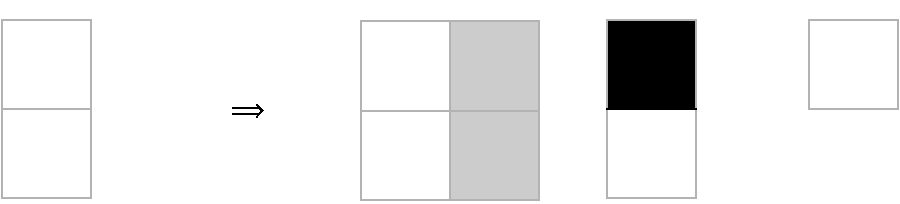
\includegraphics[ width = 4in ]{pdf/more_examples/svd_02_01_01} 
%  ` \caption{example caption}
   \label{fig:examples:21}
\end{figure}

The $\X{}$ matrix is trivial. Since it must be unitary the magnitude is one:
\begin{equation}
  \X{}= \mat{c}{1}.
\end{equation}
The lone singular value is the scale factor $r=\sqrt{2^{2}+\frac{1}{2}^{2}}$ which is the length of the vector:
\begin{equation}
  \sig{} = \mat{c}{\frac{\sqrt{5}}{2}\\0}.
\end{equation}
  For the codomain matrix we start with the image and normalize the column vector:
\begin{equation}
  \Y{}=\mat{cc}{c_{1}&c_{2}}, \qquad c_{1}=\frac{\sqrt{5}}{2}\mat{c}{2\\1}.
\end{equation}
The only quantity missing now is the null space vector $c_{2}$. Pick an orthogonal complement to $c_{1}$ and the codomain basis matrix is
\begin{equation}
  \Y{}=\frac{1}{\sqrt{5}}\mat{rr}{2&1\\1&-2}.
\end{equation}
The \svdl \ is then
\begin{equation}
  \begin{split}
    \svda{T}\\
    \mat{c}{1\\\frac{1}{2}} &= \frac{1}{\sqrt{5}}
    \mat{rr}{2&-1\\1&2}
    \mat{c}{\frac{\sqrt{5}}{2}\\0}
    \mat{c}{1}.
  \end{split}
  \label{eq:cases:2vdecomp}
\end{equation}

%%
\subsection{\vvv s}
Consider this \vvv:
\begin{equation}
  v = \mat{r}{1\\2\\-2}.
\end{equation}
The decomposition will have the shapes given by this
\begin{equation}
  \begin{array}{ccccc}
  \A{} &=& \Y{} & \sig{} & \X{T}\\
  \by{m}{n}&=&\paren{\by{m}{m}}&\paren{\by{m}{n}}&\paren{\by{n}{n}}\\
  \by{3}{1}&=&\paren{\by{3}{1}}&\paren{\by{3}{1}}&\paren{\by{1}{1}},
  \end{array}
\end{equation}
as shown here:
\begin{figure}[htbp] %  figure placement: here, top, bottom, or page
   \centering
   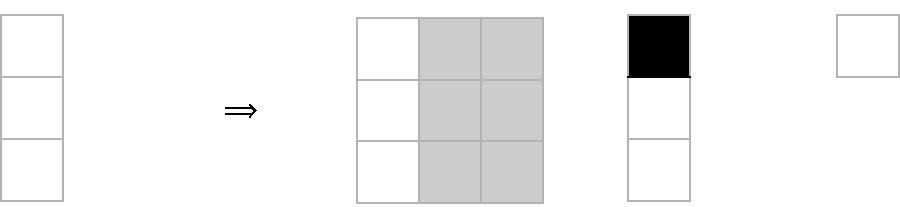
\includegraphics[ width = 4in ]{pdf/more_examples/svd_03_01_01} 
%   \caption{example caption}
   \label{fig:examples:31}
\end{figure}

We can use this vector to seed the codomain matrix:
\begin{equation}
  \Y{}_{*,1} = \frac{1}{3}\mat{r}{1\\2\\-2}.
\end{equation}
This leaves the null space vectors. A first candidate is 
\begin{equation}
  \Y{}_{*,2} = \frac{1}{\sqrt{2}}\mat{r}{0\\1\\1}.
\end{equation}
Using an inspection-based algorithm we can pick a vector like
\begin{equation}
  \Y{}_{*,3} = \frac{1}{\sqrt{18}}\mat{r}{4\\-1\\1}.
\end{equation}
The lone singular value is the length of the vector. The \svdl \ becomes
\begin{equation}
  \begin{split}
    \svda{T}\\
    \mat{r}{1\\2\\-2} &=
    \left[
\begin{array}{ r >{\columncolor{ltgray}}r >{\columncolor{ltgray}}r }
  \frac{1}{3} & 0 & \frac{4}{ \sqrt{18} } \\[5pt]
  \frac{2}{3} & \frac{1}{\sqrt{2}} & -\frac{1}{ \sqrt{18} } \\[5pt]
 -\frac{2}{3} & \frac{1}{\sqrt{2}} &  \frac{1}{ \sqrt{18} }
\end{array}
\right] 
    \left[
\begin{array}{c}
 3 \\ \hline
 0 \\
 0
\end{array}
\right]
  \mat{c}{1}.
  \end{split}
\end{equation}

The shortcut won't work. 
\begin{equation}
  v = \mat{c}{\sin\theta \\ 0 \\ \cos\theta}.
\end{equation}

\begin{equation}
  \begin{split}
    \W{y} = v v^{\mathrm{T}} &= \mat{c}{\sin\theta \\ 0 \\ \cos\theta}\mat{ccc}{\sin\theta & 0 & \cos\theta}\\
    &= \mat{ccc}{\sin^{2}\theta & 0 & \sin\theta \cos\theta\\ 0 & 0 & 0 \\ \sin\theta \cos\theta & 0 & \cos^{2}\theta}
  \end{split}
\end{equation}


Characteristic polynomial
Use cofactor expansion to compute the determinant
\begin{equation}
  \begin{split}
    p(\lambda) &= \det \paren{\W{y} - \lambda \I{3}}\\ &= 
    \det\mat{c|r|c}{\sin^{2}\theta - \lambda & 0 & \sin\theta \cos\theta\\\hline 0 & - \lambda & 0 \\ \sin\theta \cos\theta & 0 & \cos^{2}\theta- \lambda} \\
    &= \paren{\sin^{2}\theta - \lambda}\det\mat{cc}{-\lambda & 0 \\ 0 & \cos^{2}\theta- \lambda}\\ & \quad- 0 \det\mat{cc}{0 & 0 \\ \sin\theta \cos\theta & \cos^{2}\theta- \lambda}\\
     & \quad + \paren{\cos^{2}\theta - \lambda}\det\mat{cc}{0 & -\lambda \\ \sin\theta \cos\theta & 0}\\
  \end{split}
\end{equation}

The roots of the characteristic polynomial are the eigenvalues
\begin{equation}
  p(\lambda) = \lambda^{2}\paren{\lambda-1} = 0
\end{equation}
leads to the spectrum
\begin{equation}
  \lambda\paren{\W{y}} = \lst{1,0,0}.
\end{equation}
Therefore there is one singular value, 
\begin{equation}
  \sigma_{1} = 1.
\end{equation}
The eigenvector solves
\begin{equation}
  \begin{split}
    \W{y}u &= \lambda u\\
    \mat{ccc}{\sin^{2}\theta & 0 & \sin\theta \cos\theta\\ 0 & 0 & 0 \\ \sin\theta \cos\theta & 0 & \cos^{2}\theta} \mat{c}{u_{1} \\ 0 \\ u_{3}} & = \mat{c}{u_{1} \\ 0 \\ u_{3}}
  \end{split}
\end{equation}
This reduces to the system
\begin{equation}
\mat{cc}
{\sin^{2}\theta & \sin\theta \cos\theta\\
 \sin\theta \cos\theta & \cos^{2}\theta}
\mat{c}{u_{1} \\ u_{3}} = \mat{c}{u_{1} \\ u_{3}}
\end{equation}



%%
\subsection{$10-$vectors}
You can quickly verify that
\begin{equation}
  \begin{split}
    \svda{T}\\
    \mat{r}{1\\0\\0\\0\\0\\0\\0\\0\\0\\0} &=
    \left[
\begin{array}{ r >{\columncolor{ltgray}}r >{\columncolor{ltgray}}r >{\columncolor{ltgray}}r >{\columncolor{ltgray}}r >{\columncolor{ltgray}}r >{\columncolor{ltgray}}r >{\columncolor{ltgray}}r >{\columncolor{ltgray}}r >{\columncolor{ltgray}}r }
  1 & 0 & 0 & 0 & 0 & 0 & 0 & 0 & 0 & 0 \\
  0 & 1 & 0 & 0 & 0 & 0 & 0 & 0 & 0 & 0 \\
  0 & 0 & 1 & 0 & 0 & 0 & 0 & 0 & 0 & 0 \\
  0 & 0 & 0 & 1 & 0 & 0 & 0 & 0 & 0 & 0 \\
  0 & 0 & 0 & 0 & 1 & 0 & 0 & 0 & 0 & 0 \\
  0 & 0 & 0 & 0 & 0 & 1 & 0 & 0 & 0 & 0 \\
  0 & 0 & 0 & 0 & 0 & 0 & 1 & 0 & 0 & 0 \\
  0 & 0 & 0 & 0 & 0 & 0 & 0 & 1 & 0 & 0 \\
  0 & 0 & 0 & 0 & 0 & 0 & 0 & 0 & 1 & 0 \\
  0 & 0 & 0 & 0 & 0 & 0 & 0 & 0 & 0 & 1 \\
\end{array}
\right] 
    \left[
\begin{array}{c}
 1 \\ \hline
 0 \\
 0 \\
 0 \\
 0 \\
 0 \\
 0 \\
 0 \\
 0 \\
 0
\end{array}
\right]
  \mat{c}{1}.
  \end{split}
\end{equation}

This is such a simple exercise because the column vectors are already unit vectors.

A Givens rotation by an angle $\theta$ in the $4-8$ plane does not affect the decomposition because the codomain matrix $\Y{}$ is still orthogonal
\begin{equation}
  \Y{'} = 
      \left[
\begin{array}{ c >{\columncolor{ltgray}}c >{\columncolor{ltgray}}c >{\columncolor{ltgray}}c >{\columncolor{ltgray}}c >{\columncolor{ltgray}}c >{\columncolor{ltgray}}c >{\columncolor{ltgray}}c >{\columncolor{ltgray}}c >{\columncolor{ltgray}}c }
  1 & 0 & 0 & 0 & 0 & 0 & 0 & 0 & 0 & 0 \\
  0 & 1 & 0 & 0 & 0 & 0 & 0 & 0 & 0 & 0 \\
  0 & 0 & 1 & 0 & 0 & 0 & 0 & 0 & 0 & 0 \\
  0 & 0 & 0 & \cos \theta & 0 & 0 & 0 & -\sin \theta & 0 & 0 \\
  0 & 0 & 0 & 0 & 1 & 0 & 0 & 0 & 0 & 0 \\
  0 & 0 & 0 & 0 & 0 & 1 & 0 & 0 & 0 & 0 \\
  0 & 0 & 0 & 0 & 0 & 0 & 1 & 0 & 0 & 0 \\
  0 & 0 & 0 & \sin \theta & 0 & 0 & 0 & \cos \theta & 0 & 0 \\
  0 & 0 & 0 & 0 & 0 & 0 & 0 & 0 & 1 & 0 \\
  0 & 0 & 0 & 0 & 0 & 0 & 0 & 0 & 0 & 1 \\
\end{array}
\right] 
\end{equation}

Yet another rotation 1-9:
\begin{equation}
  \Y{'} = 
      \left[
\begin{array}{ c >{\columncolor{ltgray}}c >{\columncolor{ltgray}}c >{\columncolor{ltgray}}c >{\columncolor{ltgray}}c >{\columncolor{ltgray}}c >{\columncolor{ltgray}}c >{\columncolor{ltgray}}c >{\columncolor{ltgray}}c >{\columncolor{ltgray}}c }
  \cos \phi & 0 & 0 & 0 & 0 & 0 & 0 & 0 & -\sin \phi & 0 \\
  0 & 1 & 0 & 0 & 0 & 0 & 0 & 0 & 0 & 0 \\
  0 & 0 & 1 & 0 & 0 & 0 & 0 & 0 & 0 & 0 \\
  0 & 0 & 0 & \cos \theta & 0 & 0 & 0 & -\sin \theta & 0 & 0 \\
  0 & 0 & 0 & 0 & 1 & 0 & 0 & 0 & 0 & 0 \\
  0 & 0 & 0 & 0 & 0 & 1 & 0 & 0 & 0 & 0 \\
  0 & 0 & 0 & 0 & 0 & 0 & 1 & 0 & 0 & 0 \\
  0 & 0 & 0 & \sin \theta & 0 & 0 & 0 & \cos \theta & 0 & 0 \\
  \sin \phi & 0 & 0 & 0 & 0 & 0 & 0 & 0 & \cos \phi & 0 \\
  0 & 0 & 0 & 0 & 0 & 0 & 0 & 0 & 0 & 1 \\
\end{array}
\right] 
\end{equation}


\endinput

% stray commands
\newcommand{\bevrotp}[0] { \sqrt{ \half + \frac{23}{\sqrt{2341} } } }
\newcommand{\bevrotm}[0] { \sqrt{ \half - \frac{23}{\sqrt{2341} } } }

\newcommand{\oto}[0]     { \mathbf{1}^{\mathrm{T}} \mathbf{1} }
\newcommand{\xto}[0]     {          x^{\mathrm{T}} \mathbf{1} }
\newcommand{\otx}[0]     { \mathbf{1}^{\mathrm{T}} x }
\newcommand{\xtx}[0]     {          x^{\mathrm{T}} x }
 
\newcommand{\cost}[0]    { \cos \theta }
\newcommand{\sint}[0]    { \sin \theta }
\newcommand{\costs}[0]   { \cos^{2} \theta }
\newcommand{\sints}[0]   { \sin^{2} \theta }
\newcommand{\cst}[0]     { \cos \theta \sin \theta }
\newcommand{\thatmat}[0] { \mat{cc}{ \oto & \otx \\ \xto & \xtx } }

%\newcommand{\udenp}[2]   { \sqrt{#1 + \frac{#2} {\sqrt{2341}}} }
%\newcommand{\udenm}[2]   { \sqrt{#1 - \frac{#2} {\sqrt{2341}}} }
\newcommand{\udenp}[2]   { \sqrt{#1 + #2 / \sqrt{2341}} }
\newcommand{\udenm}[2]   { \sqrt{#1 - #2 / \sqrt{2341}} }
\newcommand{\urowmmp}[2] { \udenm{#1}{#2} & -\udenp{#1}{#2} }
\newcommand{\urowpmm}[2] { \udenp{#1}{#2} & -\udenm{#1}{#2} }
\newcommand{\urowppm}[2] { \udenp{#1}{#2} &  \udenm{#1}{#2} }


% bound angle
\newcommand{\bangle}[1]  { 0 \le #1 < 2\pi }

% order
\newcommand{\order}[1]   { \mathcal{o}\paren{#1} }
\newcommand{\Order}[1]   { \mathcal{O}\paren{#1} }

\newcommand{\mx}[2]      { \max\limits_{#1 \in \cmplx{ #2 }} }
\newcommand{\mn}[2]      { \min\limits_{#1 \in \cmplx{ #2 }} }

\newcommand{\mxxn}[0]    { \mx{x}{n} }
\newcommand{\mnxn}[0]    { \mn{x}{n} }

\newcommand{\mxball}[0]  { \max\limits_{\normt{x} = 1} }

% is equal?
\newcommand{\iseq}[0]    { \overset{?}{=} }

% map A
\newcommand{\mapa}[1]    { \overset{\A{#1}}{\mapsto} }

% header
\newcommand{\head}[1]    { $\A{}$ & $=$ & $\U{}$ & $\sig{}$ & $\V{*}$ }

% spacings and such
\newcommand{\wfour}[0]   {1.05in}

\endinput